% =============================================================================
% Guide complet du projet « Scoring de risque de crédit »
% Compilation (depuis docs/) : xelatex guide_projet.tex   (deux passes)
% Les chiffres viennent de chiffres.tex, généré par R/05_chiffres_document.R.
% =============================================================================
\documentclass[11pt,a4paper]{article}

\usepackage{fontspec}
\setmainfont{Charter}
\setsansfont{Avenir Next}[UprightFont=* Regular, BoldFont=* Demi Bold]
\setmonofont{Menlo}[Scale=0.85]
\usepackage[french]{babel}
\usepackage[top=2.2cm,bottom=2.2cm,left=2.4cm,right=2.4cm]{geometry}
\usepackage{amsmath,amssymb}
\usepackage{graphicx}
\graphicspath{{../resultats/figures/}{images/}}
\usepackage{booktabs,tabularx,array}
\usepackage{xcolor}
\usepackage{enumitem}
\usepackage{listings}
\usepackage[most]{tcolorbox}
\usepackage{titlesec}
\usepackage{fancyhdr}
\usepackage{tikz}
\usetikzlibrary{arrows.meta,positioning}
\usepackage{hyperref}

% Fichier généré par R/05_chiffres_document.R — ne pas modifier à la main.
\newcommand{\nBrut}{32\,581}
\newcommand{\nDoublons}{165}
\newcommand{\nFinal}{32\,409}
\newcommand{\nApprentissage}{25\,927}
\newcommand{\nTest}{6\,482}
\newcommand{\tauxDefaut}{21{,}9\,\%}
\newcommand{\nRegle}{1\,154}
\newcommand{\tauxRegle}{100{,}0\,\%}
\newcommand{\aucXgb}{0{,}923}
\newcommand{\icXgb}{[0{,}914 ; 0{,}932]}
\newcommand{\giniXgb}{0{,}847}
\newcommand{\ksXgb}{0{,}711}
\newcommand{\brierXgb}{0{,}0605}
\newcommand{\seuilXgb}{25{,}5\,\%}
\newcommand{\rappelXgb}{76{,}4\,\%}
\newcommand{\precisionXgb}{76{,}4\,\%}
\newcommand{\specXgb}{93{,}4\,\%}
\newcommand{\coutXgb}{0{,}310}
\newcommand{\aucLibre}{0{,}947}
\newcommand{\icLibre}{[0{,}940 ; 0{,}954]}
\newcommand{\rappelLibre}{83{,}4\,\%}
\newcommand{\coutLibre}{0{,}258}
\newcommand{\aucVun}{0{,}864}
\newcommand{\rappelVun}{58{,}8\,\%}
\newcommand{\precisionVun}{77{,}2\,\%}
\newcommand{\coutVun}{0{,}489}
\newcommand{\aucLogit}{0{,}876}
\newcommand{\aucGrille}{0{,}875}
\newcommand{\aucNb}{0{,}865}
\newcommand{\aucEn}{0{,}876}
\newcommand{\gainCout}{37\,\%}
\newcommand{\prixCoherence}{0{,}024}
\newcommand{\aucSansNote}{0{,}913}
\newcommand{\aucCvRetenu}{0{,}930}
\newcommand{\aucCvLibre}{0{,}947}
\newcommand{\profondeurRetenue}{7}
\newcommand{\poidsRetenu}{5}
\newcommand{\arbresRetenus}{184}
\newcommand{\aucNbGauss}{0{,}847}
\newcommand{\aucNbNoyau}{0{,}872}
\newcommand{\alphaEn}{0{,}25}
\newcommand{\cohRevenuLibre}{23{,}0\,\%}
\newcommand{\cohMontantLibre}{18{,}6\,\%}
\newcommand{\cohTauxLibre}{10{,}0\,\%}
\newcommand{\cohMontantLogit}{4{,}1\,\%}


\definecolor{bleu}{RGB}{23,66,120}
\definecolor{bleuclair}{RGB}{37,99,235}
\definecolor{gris}{RGB}{100,112,126}
\definecolor{fond}{RGB}{244,247,252}
\definecolor{vert}{RGB}{22,128,61}
\definecolor{orange}{RGB}{194,100,12}

\hypersetup{colorlinks=true, linkcolor=bleu, urlcolor=bleuclair, citecolor=bleu,
  pdftitle={Scoring de risque de crédit — guide complet du projet}, pdfauthor={Mohamed Fofana, Abdou Fall}}

\titleformat{\section}{\sffamily\Large\bfseries\color{bleu}}{\thesection}{0.8em}{}
\titleformat{\subsection}{\sffamily\large\bfseries\color{bleu}}{\thesubsection}{0.6em}{}
\titleformat{\subsubsection}{\sffamily\normalsize\bfseries}{\thesubsubsection}{0.6em}{}
\setlength{\parskip}{0.45em}
\setlength{\parindent}{0pt}
\frenchsetup{ItemLabels=\textbullet}
\setlist{itemsep=0.15em, topsep=0.3em}

\pagestyle{fancy}
\fancyhf{}
\fancyhead[L]{\sffamily\small\color{gris} Scoring de risque de crédit — guide complet}
\fancyhead[R]{\sffamily\small\color{gris}\thepage}
\renewcommand{\headrulewidth}{0.3pt}

\lstset{basicstyle=\ttfamily\small, backgroundcolor=\color{fond}, frame=single, rulecolor=\color{gris!40},
  framesep=6pt, xleftmargin=8pt, xrightmargin=8pt, breaklines=true, columns=fullflexible, keepspaces=true,
  language=R, keywordstyle=\color{bleu}\bfseries, commentstyle=\color{vert}\itshape, stringstyle=\color{orange},
  showstringspaces=false, upquote=true}

\newtcolorbox{intuition}[1][]{colback=fond, colframe=bleuclair, boxrule=0.6pt, arc=2pt, left=8pt, right=8pt,
  fonttitle=\sffamily\bfseries, title={#1}}
\newtcolorbox{alerte}[1][]{colback=orange!6, colframe=orange, boxrule=0.6pt, arc=2pt, left=8pt, right=8pt,
  fonttitle=\sffamily\bfseries, title={#1}}

\newcommand{\code}[1]{\texttt{#1}}
\newcommand{\pr}{\mathbb{P}}
\newcommand{\esp}{\mathbb{E}}

\begin{document}

% ============================== PAGE DE TITRE ==============================
\begin{titlepage}
\vspace*{2cm}
{\sffamily\color{gris}\large Projet de data science — version 2, octobre 2026}\par\vspace{0.6cm}
{\sffamily\bfseries\color{bleu}\fontsize{30}{36}\selectfont Scoring de risque\\[0.2em] de crédit}\par\vspace{0.6cm}
{\sffamily\Large Guide complet : des mathématiques à la mise en production}\par\vspace{1.2cm}
{\color{bleuclair}\rule{\linewidth}{1.2pt}}\par\vspace{0.8cm}
\newcommand{\chiffrecle}[2]{\begin{minipage}[t]{0.31\linewidth}{\sffamily\color{gris}\small #1}\par\vspace{0.35em}{\sffamily\bfseries\fontsize{26}{30}\selectfont #2}\end{minipage}}
\noindent\chiffrecle{AUC du modèle retenu}{\aucXgb}\hfill\chiffrecle{Défauts détectés}{\rappelXgb}\hfill\chiffrecle{Coût des erreurs vs v1}{$-$\gainCout}\par\vspace{1cm}
Ce document explique tout le projet, pas à pas : le problème, les données, les statistiques et les algorithmes utilisés, la façon de les évaluer honnêtement, le code, les résultats, l'application et sa mise en ligne. Chaque notion est d'abord présentée par l'intuition, puis par sa formule, puis par son rôle concret dans le projet.\par
\vfill
{\sffamily\bfseries Mohamed Fofana} \quad et \quad {\sffamily\bfseries Abdou Fall}\par
{\color{gris} Projet de Compléments de mathématiques, L3 MIASHS, Université Grenoble Alpes — repris et amélioré en 2026}\par\vspace{0.3cm}
Application : \url{https://credit-risk-app-c8ye.onrender.com}\par
Code : \url{https://github.com/Mohamed-Fof/Credit-Risk}
\end{titlepage}

\tableofcontents
\newpage

% ============================== 1. LE PROBLÈME ==============================
\section{Le problème : prêter sans se tromper}

Une banque reçoit une demande de prêt. Elle doit décider de l'accorder ou non, sans savoir si l'emprunteur remboursera. Le \emph{scoring de crédit} consiste à estimer, à partir des caractéristiques du dossier (revenu, montant demandé, historique…), la \textbf{probabilité de défaut} : la probabilité que l'emprunteur ne rembourse pas.

\begin{intuition}[Les deux erreurs n'ont pas le même prix]
Accorder un prêt à un futur défaillant (\emph{faux négatif}) fait perdre une grande partie du capital prêté. Refuser un bon client (\emph{faux positif}) ne fait perdre que la marge d'intérêt qu'il aurait rapportée. Dans ce projet, on suppose qu'un défaut accordé coûte \textbf{5 fois} plus qu'un refus à tort. Cette hypothèse guide tout le choix de la décision finale (section~\ref{sec:seuil}).
\end{intuition}

Un bon modèle de crédit doit réunir quatre qualités, et pas seulement la première :
\begin{enumerate}
\item \textbf{Discriminer} : donner un score plus risqué aux futurs défaillants qu'aux bons payeurs (mesuré par l'AUC).
\item \textbf{Être calibré} : quand il annonce 30\,\% de risque, il doit y avoir environ 30\,\% de défauts.
\item \textbf{Être cohérent} : le risque ne doit pas baisser quand on emprunte plus, ni monter quand le revenu augmente.
\item \textbf{Être explicable} : un conseiller doit pouvoir dire pourquoi un dossier est refusé.
\end{enumerate}

Ce guide montre comment chacune de ces qualités a été construite et vérifiée, et pourquoi le modèle finalement retenu n'est \emph{pas} celui qui a la meilleure AUC.

% ============================== 2. LES DONNÉES ==============================
\section{Les données}

\subsection{Source et variables}
Le jeu public \emph{Credit Risk Dataset} (Kaggle) contient \nBrut{} prêts à la consommation, avec leur issue : remboursé ou défaut. Les noms d'origine, en anglais, ont tous été traduits par un dictionnaire unique (\code{app/preparation.R}).

\begin{center}\small
\begin{tabularx}{\linewidth}{@{}l l X@{}}
\toprule
\textbf{Nom dans le projet} & \textbf{Nom d'origine} & \textbf{Signification} \\
\midrule
\code{age} & \code{person\_age} & âge de l'emprunteur \\
\code{revenu\_annuel} & \code{person\_income} & revenu annuel, en dollars \\
\code{statut\_logement} & \code{person\_home\_ownership} & locataire, propriétaire, crédit immobilier en cours, autre \\
\code{anciennete\_emploi} & \code{person\_emp\_length} & ancienneté professionnelle, en années \\
\code{motif\_pret} & \code{loan\_intent} & études, santé, création d'entreprise, personnel, travaux, regroupement de dettes \\
\code{note\_risque} & \code{loan\_grade} & note de A (meilleure) à G attribuée par le prêteur \\
\code{montant\_pret} & \code{loan\_amnt} & montant emprunté \\
\code{taux\_interet} & \code{loan\_int\_rate} & taux d'intérêt, en \% \\
\code{taux\_effort} & \emph{recalculé} & montant / revenu \\
\code{defaut\_anterieur} & \code{cb\_person\_default\_on\_file} & défaut de paiement déjà enregistré (oui/non) \\
\code{anciennete\_credit} & \code{cb\_person\_cred\_hist\_length} & ancienneté de l'historique de crédit \\
\code{defaut} & \code{loan\_status} & \textbf{cible} : 1 = défaut, 0 = remboursé \\
\bottomrule
\end{tabularx}
\end{center}

\subsection{Nettoyage}
\begin{itemize}
\item \textbf{\nDoublons{} doublons exacts} sont retirés \emph{avant} tout découpage. Sinon, un même dossier pourrait se retrouver à la fois dans les données d'apprentissage et de test : le modèle serait évalué sur un dossier qu'il a déjà vu (une \emph{fuite d'information}).
\item 5 âges supérieurs à 100 ans et 2 anciennetés professionnelles impossibles (jusqu'à 123 ans) sont retirés.
\item Le taux d'effort fourni était arrondi à deux décimales : il est recalculé exactement.
\end{itemize}
Il reste \textbf{\nFinal{} dossiers}, dont \tauxDefaut{} de défauts.

\subsection{Valeurs manquantes}
Le taux d'intérêt manque pour 9,5\,\% des dossiers et l'ancienneté pour 2,7\,\%. Ces valeurs sont remplacées par la \emph{médiane}, calculée sur les seules données d'apprentissage. Mais l'absence elle-même est une information : un dossier où le taux n'est pas renseigné n'est pas un dossier quelconque. On ajoute donc deux indicatrices, \code{taux\_manquant} et \code{anciennete\_manquante}, qui valent 1 quand la valeur était absente.

\subsection{Une découverte importante : des règles quasi déterministes}
\label{sec:regles}
En étudiant le taux de défaut selon le taux d'effort, on découvre une rupture brutale : chez les locataires notés A ou B dont le taux d'effort dépasse 32\,\%, le taux de défaut est de \textbf{\tauxRegle{}} sur \nRegle{} dossiers.

\begin{alerte}[Limite majeure du jeu de données]
Aucun portefeuille de crédit réel ne présente un seuil aussi parfait. Ce jeu de données est en partie simulé : il contient des règles qu'un modèle flexible apprend presque par cœur. Les performances obtenues ici sont donc \emph{optimistes} et ne se transposeraient pas telles quelles à une banque. C'est la première chose à dire en entretien quand on présente ce projet.
\end{alerte}

% ============================== 3. PROTOCOLE ==============================
\section{Le protocole : évaluer sans se mentir}

L'erreur la plus fréquente en data science n'est pas un mauvais modèle, c'est une \emph{évaluation trop optimiste}. Le protocole sert à garantir que les chiffres annoncés valent pour des dossiers que le modèle n'a jamais vus.

\subsection{Découpage apprentissage / test}
Les données sont séparées en deux, \emph{avant toute autre transformation} :
\begin{itemize}
\item \textbf{apprentissage} (\nApprentissage{} dossiers, 80\,\%) : sert à tout — régler, entraîner, choisir le seuil ;
\item \textbf{test} (\nTest{} dossiers, 20\,\%) : mis sous clé, utilisé \emph{une seule fois}, à la toute fin.
\end{itemize}
Le découpage est \textbf{stratifié} : le taux de défaut est le même des deux côtés (21,9\,\%). Sans cela, un tirage malheureux pourrait mettre plus de défauts d'un côté et fausser la comparaison.

\subsection{Validation croisée à 5 plis}
Pour régler les modèles sans toucher au test, l'échantillon d'apprentissage est découpé en 5 parts (\emph{plis}) stratifiées. On entraîne sur 4 plis et on prédit le cinquième, cinq fois de suite. Chaque dossier d'apprentissage reçoit ainsi une prédiction \emph{hors pli}, faite par un modèle qui ne l'a pas vu.

\begin{center}
\begin{tikzpicture}[x=1.9cm, y=0.5cm, font=\sffamily\scriptsize]
\foreach \i in {1,...,5} {
  \foreach \j in {1,...,5} {
    \ifnum\i=\j \fill[orange!70] (\j-1, -\i) rectangle (\j-0.06, -\i+0.8);
    \else \fill[bleuclair!45] (\j-1, -\i) rectangle (\j-0.06, -\i+0.8); \fi
  }
  \node[anchor=east] at (-0.1, -\i+0.4) {tour \i};
}
\fill[bleuclair!45] (5.3,-2) rectangle (5.5,-1.5); \node[anchor=west] at (5.55,-1.75) {apprentissage};
\fill[orange!70] (5.3,-3.2) rectangle (5.5,-2.7); \node[anchor=west] at (5.55,-2.95) {prédiction};
\end{tikzpicture}
\end{center}

Deux précautions rendent ce protocole rigoureux :
\begin{itemize}
\item les \textbf{mêmes plis} servent à tous les modèles : la comparaison est équitable ;
\item la \textbf{préparation est réapprise dans chaque pli} : la médiane utilisée pour imputer est calculée sur les 4 plis d'entraînement, jamais sur le pli prédit.
\end{itemize}
Toutes les étapes aléatoires utilisent la graine 2026 : relancer le projet redonne exactement les mêmes chiffres.

% ============================== 4. MODÈLES ==============================
\section{Les modèles : intuitions et mathématiques}

Six modèles sont comparés, du plus simple au plus flexible. On note $x \in \mathbb{R}^p$ les caractéristiques d'un dossier et $Y \in \{0,1\}$ le défaut.

\subsection{Régression logistique}
\begin{intuition}[Intuition]
On additionne les effets des variables sur une échelle « log-cote », puis on transforme ce total en probabilité comprise entre 0 et 1.
\end{intuition}
Le modèle s'écrit
\[
\pr(Y=1 \mid x) = \sigma(\beta_0 + \beta^\top x), \qquad \sigma(z) = \frac{1}{1+e^{-z}}.
\]
La quantité $\log\frac{p}{1-p}$ est la \emph{log-cote} (log-odds) : elle est linéaire en $x$. Ainsi $e^{\beta_j}$ est le \emph{rapport de cotes} : de combien la cote de défaut est multipliée quand $x_j$ augmente d'une unité. Les coefficients maximisent la log-vraisemblance
\[
\ell(\beta) = \sum_{i=1}^n \big[ y_i \log p_i + (1-y_i)\log(1-p_i) \big],
\]
par l'algorithme de Newton-Raphson (moindres carrés repondérés itérés). Dans le projet, le revenu et le montant entrent en logarithme, car leur effet est proportionnel plutôt qu'additif, et les variables qualitatives sont codées en indicatrices.

\subsection{Logistique pénalisée (elastic net)}
Pour éviter le sur-apprentissage et sélectionner les variables utiles, on ajoute une pénalité :
\[
\hat\beta = \arg\min_\beta \; -\frac{1}{n}\ell(\beta) + \lambda\Big[\frac{1-\alpha}{2}\lVert\beta\rVert_2^2 + \alpha\lVert\beta\rVert_1\Big].
\]
La partie $\lVert\beta\rVert_1$ (lasso) peut annuler des coefficients ; la partie $\lVert\beta\rVert_2^2$ (ridge) stabilise les variables corrélées. $\alpha$ et $\lambda$ sont choisis par validation croisée (ici $\alpha = \alphaEn$). Résultat : même performance que la logistique simple ($\aucEn$), ce qui montre que la logistique ne sur-apprenait pas — sa limite est sa \emph{forme} linéaire, pas son nombre de paramètres.

\subsection{Naïve Bayes}
Par la formule de Bayes, et en supposant les variables indépendantes conditionnellement à la classe :
\[
\pr(Y=k \mid x) \;\propto\; \pr(Y=k)\prod_{j=1}^p f_j(x_j \mid Y=k).
\]
L'hypothèse d'indépendance est fausse ici (le taux d'effort dépend du montant et du revenu), d'où des probabilités moins bien calibrées. Pour les variables numériques, la densité $f_j$ est estimée par \textbf{noyau} plutôt que par une loi normale :
\[
\hat f(x) = \frac{1}{nh}\sum_{i=1}^n K\Big(\frac{x - x_i}{h}\Big),
\]
ce qui épouse les distributions asymétriques (revenu, montant). Gain mesuré en validation croisée : AUC \aucNbNoyau{} contre \aucNbGauss{} avec une loi normale.

\subsection{Grille de score bancaire}
C'est la méthode historique des banques, appréciée parce qu'un conseiller peut la lire.
\begin{enumerate}
\item \textbf{Discrétisation} : chaque variable est découpée en classes (par exemple, taux d'effort $<10\,\%$, $10$–$20\,\%$…), choisies par un arbre de décision.
\item \textbf{Poids de l'évidence (WoE)} de la classe $i$ :
\[
\mathrm{WoE}_i = \ln\frac{D_i / D}{N_i / N},
\]
où $D_i$ et $N_i$ comptent les défauts et non-défauts de la classe, $D$ et $N$ les totaux. Un WoE positif signale une classe plus risquée que la moyenne.
\item \textbf{Valeur d'information} d'une variable : $\mathrm{IV} = \sum_i \big(\frac{D_i}{D} - \frac{N_i}{N}\big)\mathrm{WoE}_i$. On ne garde que les variables d'IV supérieure à 0,02.
\item \textbf{Régression logistique sur les WoE}, puis conversion en points :
\[
\text{score} = A - B\ln(\text{cote}), \qquad B = \frac{\text{PDO}}{\ln 2}, \qquad A = 600 + B\ln\tfrac{1}{19}.
\]
600 points correspondent à une cote de 1 contre 19 (5\,\% de risque), et chaque tranche de 50 points (PDO, \emph{points to double the odds}) divise la cote par deux. Chaque classe reçoit $-B\,\beta_j\,\mathrm{WoE}_{ij}$ points.
\end{enumerate}

\begin{alerte}[Règle des signes]
Tous les coefficients de la logistique sur WoE doivent être positifs. Ici, le défaut antérieur obtenait un coefficient négatif, car son information est déjà contenue dans la note du prêteur (colinéarité) : un défaut antérieur \emph{rapportait} des points. La variable a été retirée et le modèle réestimé, comme le veut la pratique bancaire. Un test automatique vérifie aussi qu'un taux d'effort plus élevé ne rapporte jamais de points.
\end{alerte}

\subsection{Gradient boosting (XGBoost)}
\begin{intuition}[Intuition]
On construit une suite de petits arbres de décision. Chaque nouvel arbre corrige les erreurs de la somme des précédents. La prédiction est la somme de tous les arbres.
\end{intuition}
Le modèle est additif, sur l'échelle log-cote : $F(x) = \sum_{m=1}^M f_m(x)$, où chaque $f_m$ est un arbre. On minimise
\[
\mathcal{L} = \sum_{i} l\big(y_i, F(x_i)\big) + \sum_m \Omega(f_m), \qquad \Omega(f) = \gamma T + \tfrac{1}{2}\lambda \lVert w \rVert^2,
\]
où $l$ est la perte logistique, $T$ le nombre de feuilles et $w$ leurs valeurs. À l'étape $m$, XGBoost approche la perte par un développement de Taylor d'ordre 2, avec $g_i$ et $h_i$ les dérivées première et seconde de $l$ en $F_{m-1}(x_i)$. Pour une feuille contenant les dossiers $I_j$, la valeur optimale et le gain d'une coupure valent
\[
w_j^\star = -\frac{\sum_{i\in I_j} g_i}{\sum_{i\in I_j} h_i + \lambda}, \qquad
\text{gain} = \frac12\Big[\frac{G_G^2}{H_G+\lambda} + \frac{G_D^2}{H_D+\lambda} - \frac{(G_G+G_D)^2}{H_G+H_D+\lambda}\Big] - \gamma .
\]
Chaque arbre est ajouté avec un \emph{taux d'apprentissage} $\eta = 0{,}05$ : $F_m = F_{m-1} + \eta f_m$. On sous-échantillonne 80\,\% des dossiers et des variables à chaque arbre, et le nombre d'arbres est fixé par \textbf{arrêt précoce} : on s'arrête quand l'AUC de validation croisée ne progresse plus depuis 100 arbres.

\subsubsection*{Contraintes de monotonie}
On peut imposer qu'une prédiction soit monotone en une variable : XGBoost refuse alors toute coupure dont les deux branches violeraient l'ordre, et propage des bornes aux sous-arbres. Le modèle retenu impose que, toutes choses égales par ailleurs, le risque \emph{croisse} avec le montant, le taux d'effort, le taux d'intérêt, la note et un défaut antérieur, et \emph{décroisse} avec le revenu. La section~\ref{sec:coherence} explique pourquoi c'est indispensable.

Réglage retenu (validation croisée, 12 combinaisons) : profondeur \profondeurRetenue, poids minimal par feuille \poidsRetenu, \arbresRetenus{} arbres.

% ============================== 5. ÉVALUATION ==============================
\section{Mesurer la performance}

\subsection{AUC, Gini et KS}
\textbf{L'AUC} est l'aire sous la courbe ROC. Elle a une interprétation très concrète : c'est la probabilité qu'un futur défaillant tiré au hasard reçoive un score plus risqué qu'un bon payeur tiré au hasard. On la calcule exactement par la statistique de Mann-Whitney :
\[
\mathrm{AUC} = \frac{R_1 - n_1(n_1+1)/2}{n_1\,n_0},
\]
où $R_1$ est la somme des rangs des scores des défauts, $n_1$ et $n_0$ les effectifs. 0,5 correspond au hasard, 1 à un classement parfait.

Les banques utilisent le \textbf{Gini} $= 2\,\mathrm{AUC} - 1$ et le \textbf{KS}, écart maximal entre les fonctions de répartition des scores des deux populations : $\mathrm{KS} = \max_s |F_1(s) - F_0(s)|$.

\subsection{Calibration : score de Brier}
L'AUC ne regarde que l'ordre des scores, pas leur valeur. Le \textbf{score de Brier}, $\frac1n\sum_i (p_i - y_i)^2$, mesure si les probabilités sont justes. La courbe de calibration compare, par décile, la probabilité moyenne annoncée au taux de défaut réellement observé.

\subsection{Intervalles de confiance et test de DeLong}
L'AUC mesurée sur \nTest{} dossiers est une estimation : la méthode de DeLong fournit sa variance, donc un intervalle de confiance à 95\,\%. Elle permet aussi de tester si deux modèles diffèrent vraiment sur les mêmes dossiers (test apparié). Tous les écarts entre le modèle retenu et les modèles linéaires sont significatifs ($p < 0{,}0001$).

\subsection{Du score à la décision : le seuil}
\label{sec:seuil}
Le modèle donne une probabilité $p$ ; il faut décider : refuser si $p \geq s$. Le seuil $s = 0{,}5$ de la version 1 laissait passer 41\,\% des défauts. On choisit plutôt le seuil qui minimise le coût moyen
\[
C(s) = \frac{1}{n}\big[\,5 \cdot \mathrm{FN}(s) + 1 \cdot \mathrm{FP}(s)\,\big].
\]
\begin{intuition}[Le seuil théorique]
Pour un modèle parfaitement calibré, refuser coûte $(1-p)\cdot 1$ (on perd un bon client avec probabilité $1-p$) et accepter coûte $p \cdot 5$. On refuse donc dès que $5p > 1-p$, soit $p > 1/6 \approx 16{,}7\,\%$. Le seuil réellement retenu (\seuilXgb) est cherché numériquement sur les prédictions hors pli, \emph{jamais} sur le test, pour tenir compte des imperfections de calibration.
\end{intuition}

% ============================== 6. EXPLICABILITÉ ==============================
\section{Expliquer chaque décision : les valeurs de Shapley}

Un modèle à plusieurs centaines d'arbres n'est pas lisible directement. Les \textbf{valeurs de Shapley}, issues de la théorie des jeux coopératifs, répartissent la prédiction entre les variables de façon équitable. La contribution de la variable $j$ est sa contribution marginale moyenne sur tous les ordres d'arrivée possibles des variables :
\[
\phi_j = \sum_{S \subseteq N\setminus\{j\}} \frac{|S|!\,(|N|-|S|-1)!}{|N|!}\,\big[v(S\cup\{j\}) - v(S)\big].
\]
Propriété clé (\emph{efficacité}) : la somme des contributions, plus une valeur de base, redonne exactement la prédiction en log-cote,
\[
F(x) = \phi_0 + \sum_{j} \phi_j .
\]
Pour les arbres, l'algorithme TreeSHAP calcule ces valeurs exactement et rapidement. Dans l'application, chaque dossier affiche ses contributions : en rouge ce qui augmente le risque, en vert ce qui le réduit. Un test automatique vérifie la propriété d'efficacité.

% ============================== 7. RÉSULTATS ==============================
\section{Résultats}

\subsection{Tableau général}
Mesures sur les \nTest{} dossiers de test, jamais utilisés auparavant.

\begin{center}\small
\begin{tabular}{@{}lcccccc@{}}
\toprule
\textbf{Modèle} & \textbf{AUC} & \textbf{IC 95\,\%} & \textbf{Défauts détectés} & \textbf{Refus justifiés} & \textbf{Coût} \\
\midrule
\textbf{XGBoost contraint (retenu)} & \textbf{\aucXgb} & \icXgb & \textbf{\rappelXgb} & \textbf{\precisionXgb} & \textbf{\coutXgb} \\
XGBoost non contraint & \aucLibre & \icLibre & \rappelLibre & — & \coutLibre \\
Régression logistique & \aucLogit & & & & \\
Elastic net & \aucEn & & & & \\
Grille de score & \aucGrille & & & & \\
Naïve Bayes & \aucNb & & & & \\
\emph{Logistique v1 (soutenance)} & \emph{\aucVun} & & \emph{\rappelVun} & \emph{\precisionVun} & \emph{\coutVun} \\
\bottomrule
\end{tabular}
\end{center}
Le tableau complet (Gini, KS, Brier, spécificité…) est dans \code{resultats/metriques\_test.csv} et dans l'onglet « Comparaison des modèles » de l'application.

\begin{center}
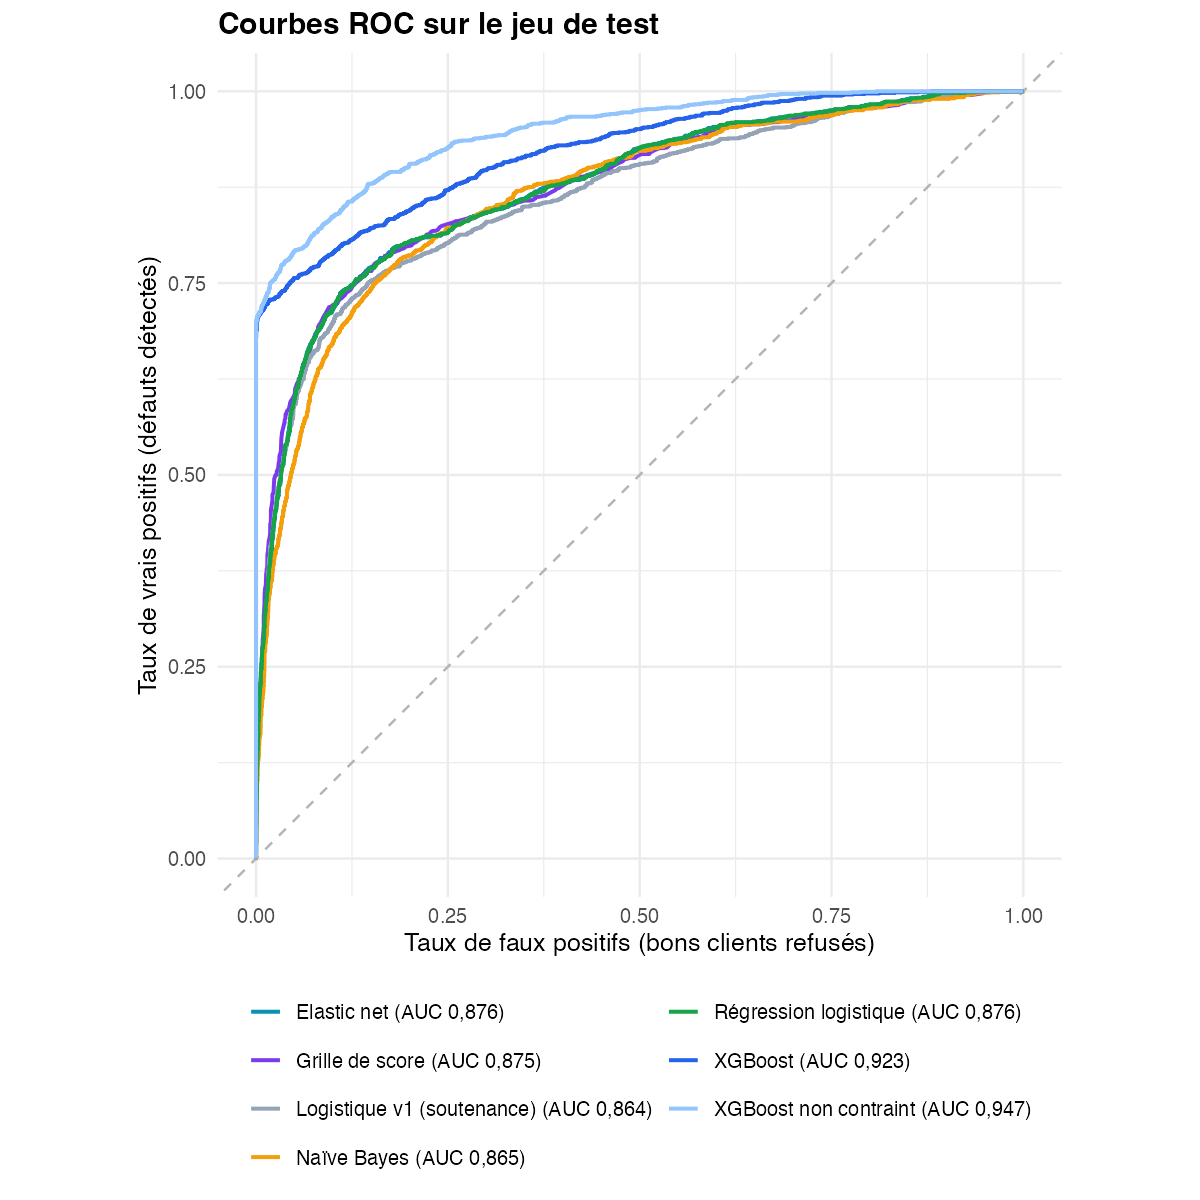
\includegraphics[width=0.49\linewidth]{roc_test.png}\hfill
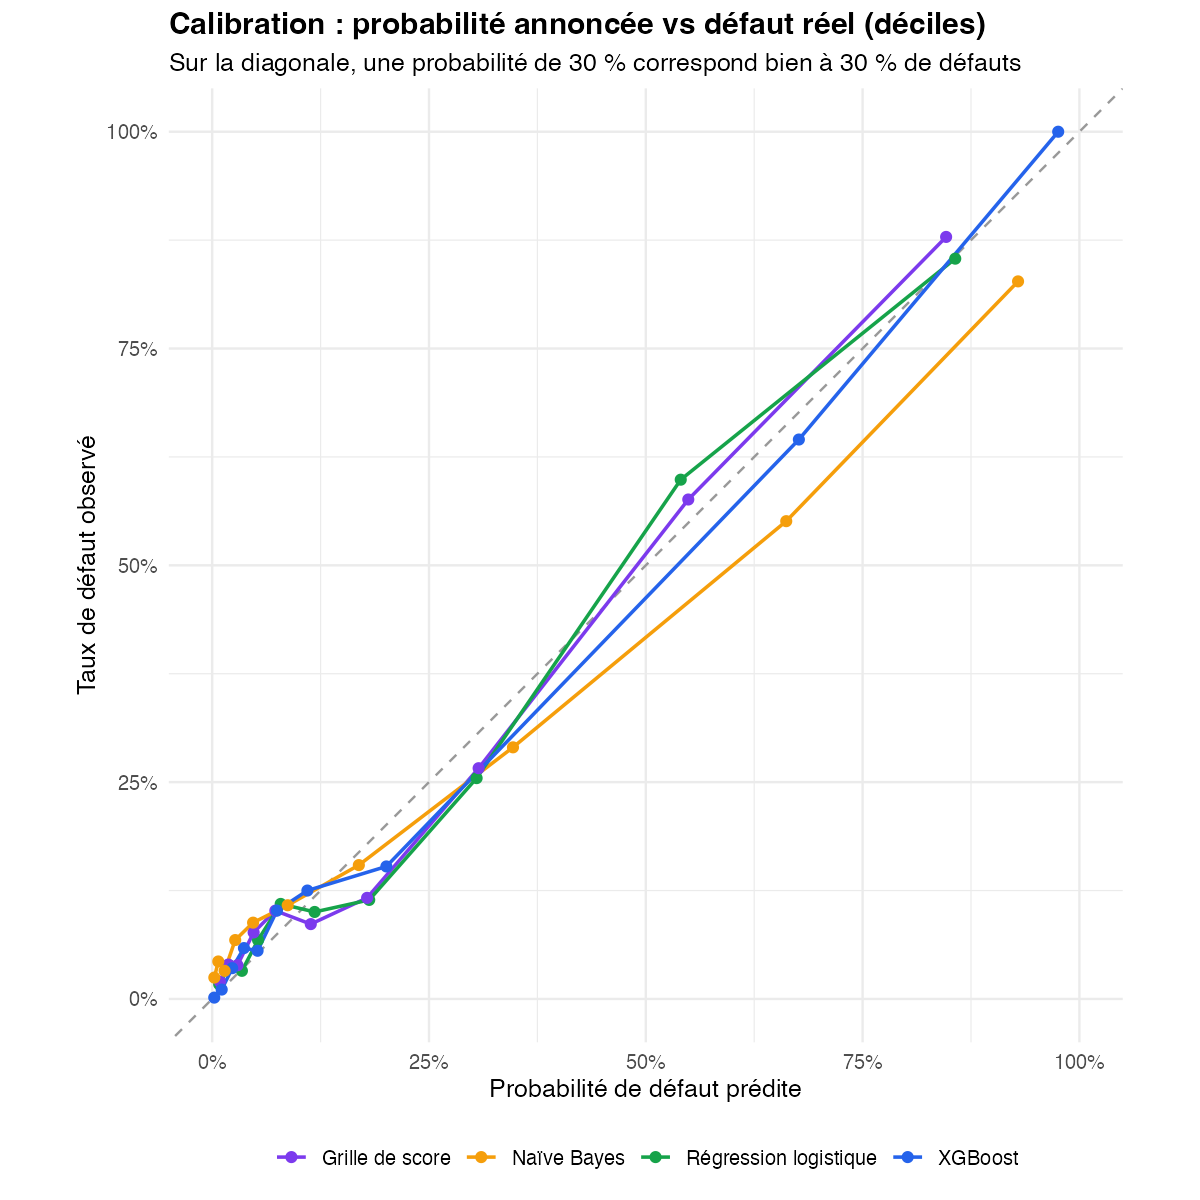
\includegraphics[width=0.49\linewidth]{calibration.png}
\end{center}

\subsection{Pourquoi le modèle retenu n'a pas la meilleure AUC}
\label{sec:coherence}
Sans contrainte, XGBoost atteint \aucLibre. Mais un audit de cohérence change tout : on modifie \emph{une seule} caractéristique de chaque dossier de test et on regarde si le risque bouge dans le bon sens.

\begin{center}\small
\begin{tabular}{@{}lccc@{}}
\toprule
\textbf{Dossiers à contresens (écart $>$ 1 point)} & \textbf{Montant +20\,\%} & \textbf{Revenu +20\,\%} & \textbf{Taux +2 points} \\
\midrule
XGBoost non contraint & \cohMontantLibre & \cohRevenuLibre & \cohTauxLibre \\
Régression logistique & \cohMontantLogit & 0\,\% & 0\,\% \\
\textbf{XGBoost contraint (retenu)} & \textbf{0\,\%} & \textbf{0\,\%} & \textbf{0\,\%} \\
\bottomrule
\end{tabular}
\end{center}

Sans contrainte, le modèle juge un emprunteur \emph{plus risqué quand son revenu augmente} pour \cohRevenuLibre{} des dossiers : il a appris le bruit des données (le taux de défaut observé n'est pas monotone en revenu, par simple hasard d'échantillonnage). Un tel modèle n'est ni crédible pour un utilisateur, ni défendable devant un régulateur. Les contraintes coûtent \prixCoherence{} d'AUC (de \aucLibre{} à \aucXgb) : c'est le \textbf{prix de la cohérence}, et il est assumé.

Une variante a été testée : retirer le revenu brut (il reste présent via le taux d'effort) pour garantir la cohérence sans contrainte sur le revenu. L'AUC tombe alors à 0,884 : le revenu apporte une information propre, la contrainte est la bonne solution.

\subsection{La note du prêteur est-elle indispensable ?}
La note A à G est attribuée par le prêteur lui-même : l'utiliser revient en partie à recopier son avis. Sans elle, le modèle retenu atteint encore une AUC de \textbf{\aucSansNote} : il apprend réellement des caractéristiques de l'emprunteur et du prêt.

\subsection{Ce qui compte pour le modèle}
\begin{center}
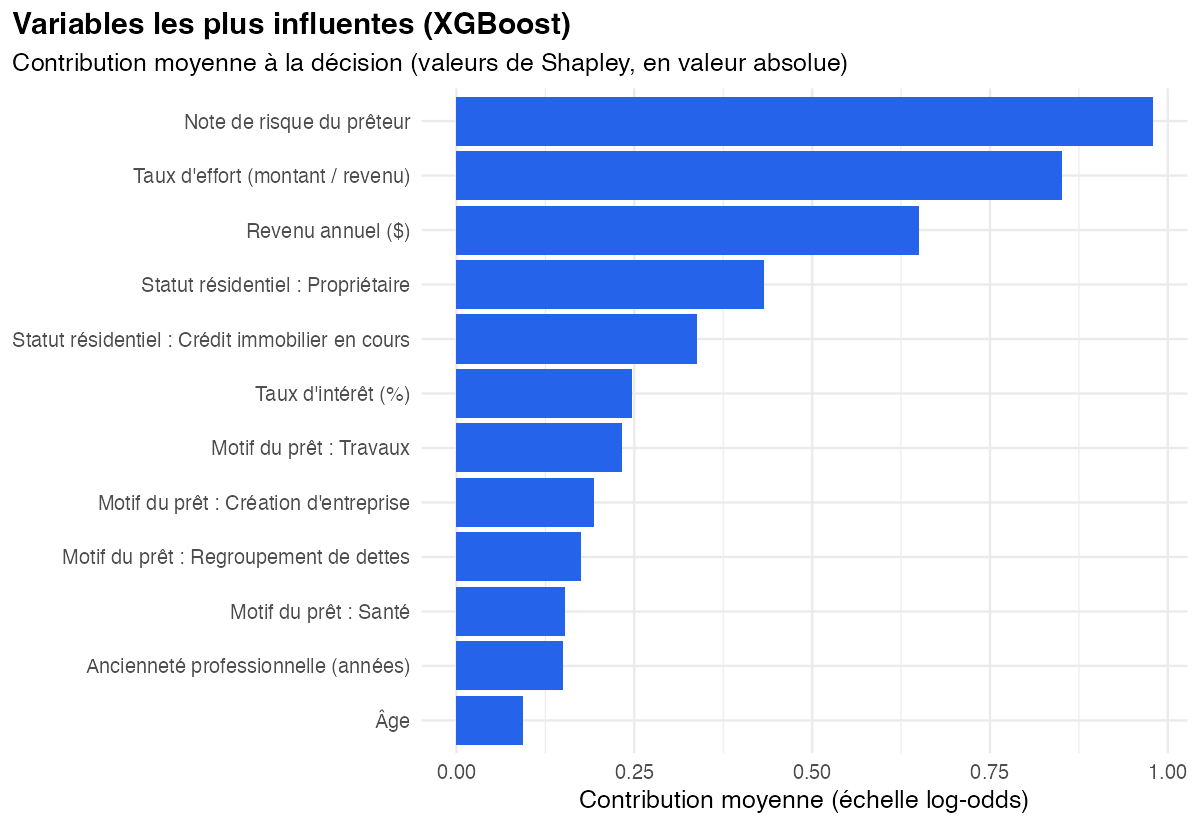
\includegraphics[width=0.72\linewidth]{importance_xgboost.png}
\end{center}
La note du prêteur, le taux d'effort et le revenu dominent, suivis du statut résidentiel : les propriétaires font beaucoup moins défaut que les locataires.

% ============================== 8. CODE ==============================
\section{Le code : organisation et bonnes pratiques}

\subsection{Architecture}
\begin{center}
\begin{tikzpicture}[node distance=0.55cm and 0.5cm, font=\sffamily\small,
  boite/.style={draw=bleu, fill=fond, rounded corners=2pt, minimum width=3.1cm, minimum height=0.9cm, align=center},
  fleche/.style={-{Stealth[length=2.2mm]}, color=bleu, thick}]
\node[boite] (d) {données brutes\\\scriptsize\code{donnees/}};
\node[boite, right=of d] (p) {01 préparation\\\scriptsize nettoyage, découpage};
\node[boite, right=of p] (m) {02 modélisation\\\scriptsize réglage, validation};
\node[boite, below=of m] (e) {03 évaluation\\\scriptsize test, figures, audit};
\node[boite, left=of e] (x) {04 export\\\scriptsize modèles allégés};
\node[boite, left=of x] (a) {application\\\scriptsize\code{app/}};
\draw[fleche] (d) -- (p); \draw[fleche] (p) -- (m); \draw[fleche] (m) -- (e); \draw[fleche] (e) -- (x); \draw[fleche] (x) -- (a);
\end{tikzpicture}
\end{center}
Une seule commande reproduit tout, en trois minutes environ : \code{Rscript R/executer\_tout.R}.

\subsection{Une source unique pour la préparation}
Le piège classique de la mise en production est l'écart entre la préparation faite à l'entraînement et celle faite dans l'application. Ici, \code{app/preparation.R} est utilisé \emph{par les deux} :
\begin{lstlisting}
appliquer_preparation <- function(df, params) {
  # L'absence d'information est conservée comme information
  df$taux_manquant <- as.integer(is.na(df$taux_interet))
  df$taux_interet[is.na(df$taux_interet)] <- params$mediane_taux
  df$taux_effort <- df$montant_pret / df$revenu_annuel
  ...
}
\end{lstlisting}
L'export vérifie ensuite que l'application reproduit \emph{exactement} (à $10^{-6}$ près) les prédictions de l'entraînement sur les \nTest{} dossiers de test.

\subsection{Chaque modèle comme un couple de fonctions}
Tous les modèles se décrivent de la même façon : une fonction \code{ajuster} et une fonction \code{predire}. La validation croisée devient alors générique, et la préparation est réapprise dans chaque pli :
\begin{lstlisting}
hors_pli <- function(modele) {
  p <- numeric(nrow(apprentissage))
  for (k in 1:5) {
    m <- modele$ajuster(apprentissage[plis != k, ])
    p[plis == k] <- modele$predire(m, apprentissage[plis == k, ])
  }
  p
}
\end{lstlisting}

\subsection{Tests automatiques}
\code{tests/tests.R} contient 26 tests, à relancer avant chaque mise en ligne : contrôle des saisies (y compris malveillantes), préparation, reproduction exacte des prédictions, additivité des valeurs de Shapley, cohérence du modèle sur \emph{tous} les dossiers de test, cohérence de la grille de score.

% ============================== 9. APPLICATION ==============================
\section{L'application : mode d'emploi}

\subsection{Utilisation}
L'application compte quatre onglets.
\begin{itemize}
\item \textbf{Simulateur} : on saisit un dossier à gauche ; l'application affiche la décision recommandée, la probabilité de défaut, l'explication de la décision et le score de la grille bancaire détaillé point par point, ainsi que l'avis des cinq modèles. Le calcul se relance automatiquement 0,4 seconde après la dernière saisie.
\item \textbf{Comparaison des modèles} : performances, courbes ROC, calibration, importance des variables, audit de cohérence.
\item \textbf{Exploration des données} : distributions et taux de défaut par modalité.
\item \textbf{Méthode} : protocole, hypothèses et limites.
\end{itemize}

\begin{center}
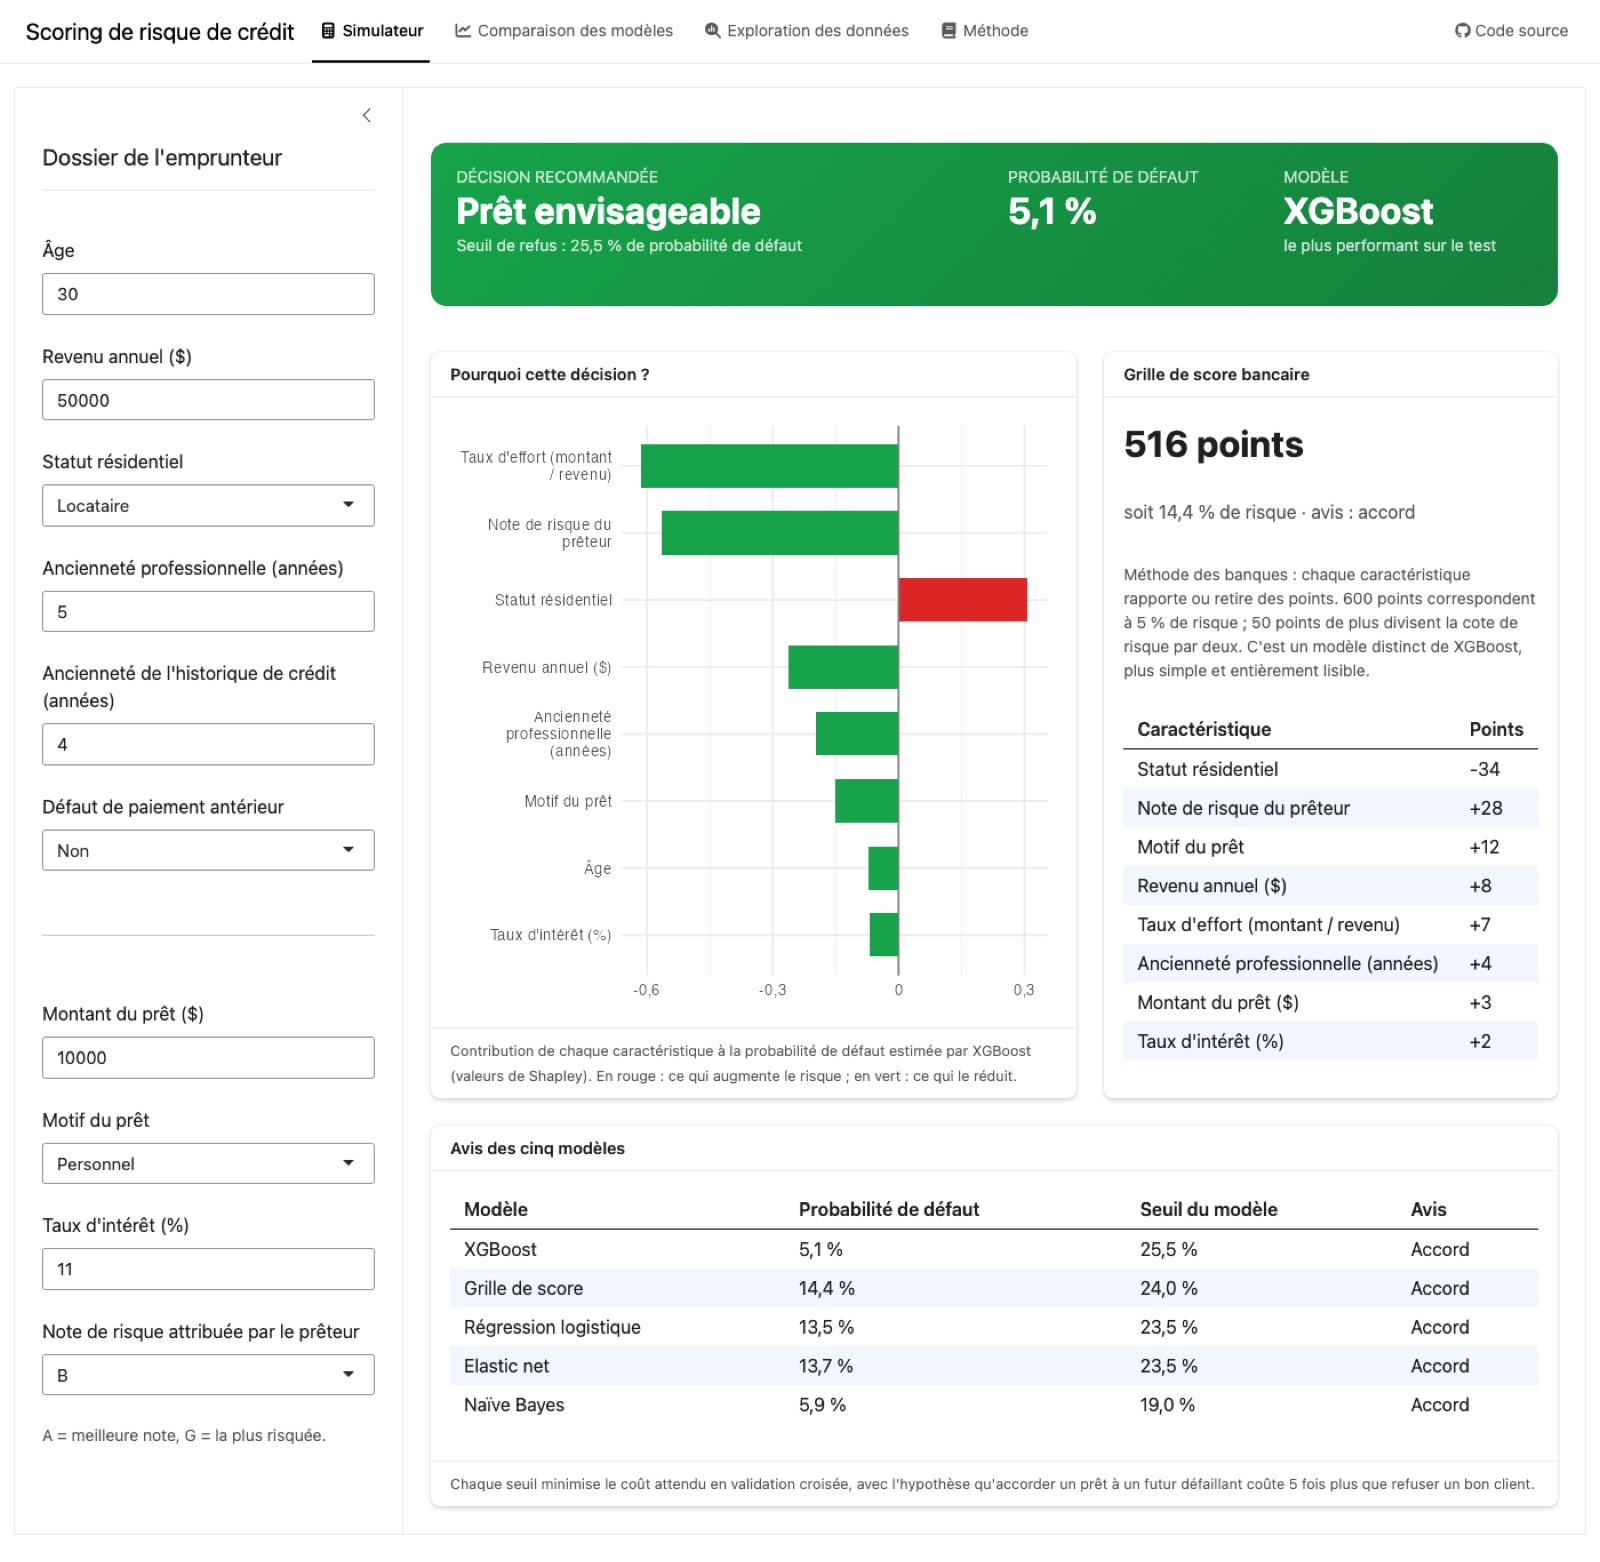
\includegraphics[width=\linewidth]{app_simulateur.jpg}\\[0.3em]
{\small\color{gris} Le simulateur : décision, explication par les valeurs de Shapley, grille de score, avis des modèles.}
\end{center}

\begin{center}
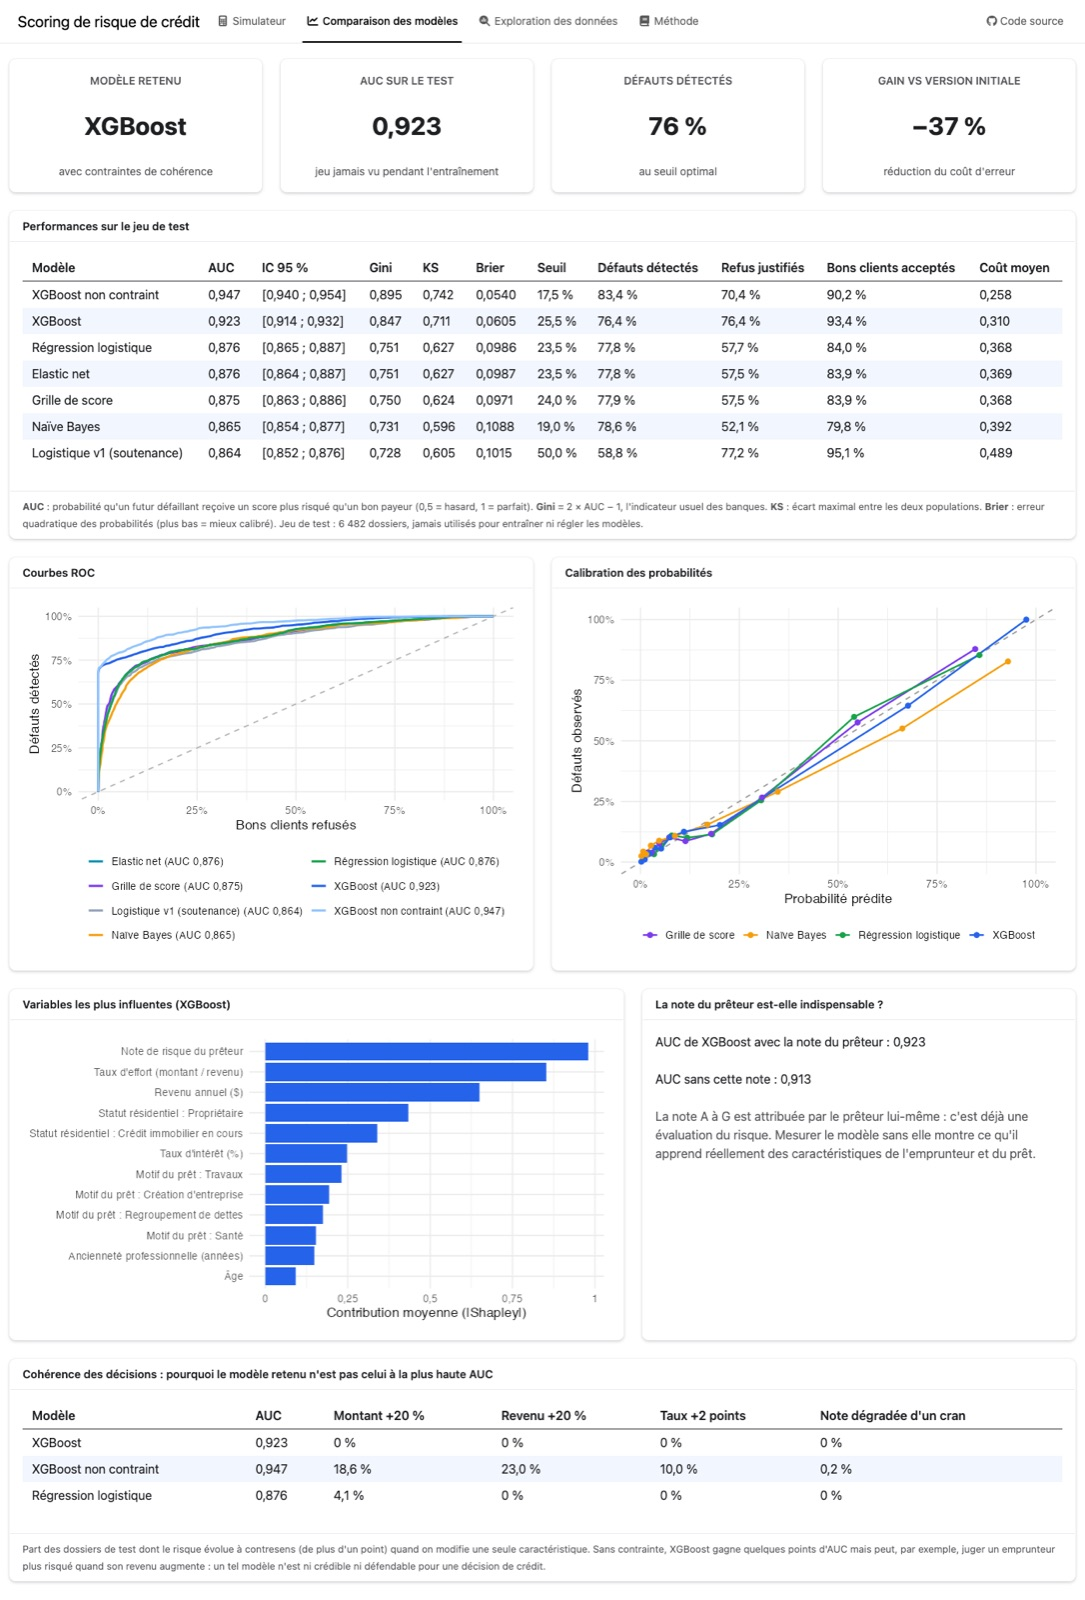
\includegraphics[width=0.78\linewidth]{app_comparaison.jpg}\\[0.3em]
{\small\color{gris} L'onglet de comparaison des modèles.}
\end{center}

\subsection{Contrôles et sécurité}
\begin{itemize}
\item \textbf{Saisies revérifiées côté serveur.} Shiny ne contrôle pas que la valeur d'une liste déroulante fait partie des choix proposés : un client modifié peut envoyer n'importe quoi. Chaque valeur est donc revérifiée (liste blanche, type, bornes, cohérence âge / ancienneté / historique, montant / revenu). Cinq attaques ont été simulées depuis un navigateur modifié (HTML piégé, code R, valeur vide, tableau, nombre géant) : toutes sont bloquées.
\item \textbf{Extrapolation signalée} : une valeur hors de l'intervalle observé à l'entraînement déclenche un avertissement.
\item \textbf{Erreurs masquées} : l'utilisateur ne voit jamais de message technique (option \code{shiny.\allowbreak sanitize.\allowbreak errors}).
\item \textbf{Aucune donnée conservée} : les dossiers saisis ne sont ni enregistrés ni transmis.
\end{itemize}

% ============================== 10. PRODUCTION ==============================
\section{La mise en production}

\subsection{Le conteneur Docker}
L'application est empaquetée dans une image Docker, une « boîte » qui contient R, les paquets et le code, et qui tourne à l'identique partout.
\begin{lstlisting}[language=bash]
FROM rocker/r-ver:4.5.1                      # R minimal (365 Mo)
RUN R -e "install.packages(c('shiny','bslib','ggplot2','xgboost','naivebayes'))"
COPY app/ /app/                              # 2,3 Mo de modèles
USER appli                                   # pas de droits administrateur
CMD Rscript -e "shiny::runApp('/app', host='0.0.0.0', port=...)"
\end{lstlisting}
Choix faits pour démarrer vite :
\begin{itemize}
\item image minimale (365 Mo contre 580 Mo pour l'image Shiny complète de la version 1) ;
\item paquets \emph{précompilés} (Posit Package Manager), figés à la date d'entraînement : la version de XGBoost qui lit le modèle est celle qui l'a créé ;
\item modèles allégés : 2,3 Mo chargés une fois au démarrage, contre un modèle de 40 Mo rechargé à chaque prédiction dans la version 1. L'application est prête en moins de 2 secondes une fois le conteneur lancé.
\end{itemize}

\subsection{Render et le cycle de mise à jour}
Render (offre gratuite) surveille le dépôt GitHub. À chaque \code{git push} sur la branche principale : construction de l'image à partir du \code{Dockerfile}, lancement du conteneur, bascule du trafic. Mettre à jour l'application, c'est donc : modifier le code, relancer \code{R/executer\_tout.R} et \code{tests/tests.R}, puis pousser.

\begin{alerte}[Le réveil de l'offre gratuite]
Render endort le service après 15 minutes sans visite, et le réveil prenait 72 secondes : un recruteur aurait attendu plus d'une minute. Une tâche GitHub Actions (\code{.github/workflows/reveil-render.yml}) appelle l'application toutes les 10 minutes pour la garder éveillée. Contrepartie : le service tourne en continu, ce qui consomme les 750 heures gratuites mensuelles de Render.
\end{alerte}

% ============================== 11. LIMITES ==============================
\section{Limites et pistes}
\begin{itemize}
\item \textbf{Données en partie simulées} (section~\ref{sec:regles}) : les performances sont optimistes. Sur des données réelles, une AUC de 0,75 à 0,85 serait déjà bonne.
\item \textbf{Pas de dimension temporelle} : impossible de vérifier la stabilité du modèle dans le temps. En banque, on validerait sur une période postérieure (\emph{out-of-time}) et on surveillerait la dérive des données en production (indice de stabilité de population, PSI).
\item \textbf{Hypothèse de coût} : le ratio 5 pour 1 devrait être calibré sur les pertes réelles (probabilité de défaut $\times$ perte en cas de défaut).
\item \textbf{Équité} : l'âge est utilisé, alors que c'est un critère sensible. Une suite naturelle serait de mesurer l'écart de décisions entre groupes d'âge et l'impact de son retrait.
\item \textbf{Usage} : l'application est un outil pédagogique, pas une décision de crédit.
\end{itemize}

% ============================== 12. GLOSSAIRE ==============================
\section{Glossaire}
\begin{description}[style=nextline, leftmargin=1.2em, font=\sffamily\bfseries\color{bleu}]
\item[AUC] probabilité qu'un défaillant reçoive un score plus risqué qu'un bon payeur.
\item[Calibration] accord entre probabilités annoncées et fréquences observées.
\item[Contrainte de monotonie] obligation pour le modèle de faire varier le risque toujours dans le même sens avec une variable.
\item[Fuite d'information] information du jeu de test qui s'infiltre dans l'entraînement et rend l'évaluation trop optimiste.
\item[Hors pli] prédiction faite par un modèle qui n'a pas vu le dossier.
\item[Log-cote] $\log\frac{p}{1-p}$, échelle sur laquelle les effets s'additionnent.
\item[Valeurs de Shapley] répartition équitable d'une prédiction entre les variables.
\item[WoE / IV] poids de l'évidence d'une classe et pouvoir discriminant d'une variable, outils des grilles de score.
\end{description}

\vspace{1em}
{\small\color{gris} Reproduire ce document : \code{Rscript R/executer\_tout.R}, puis \code{Rscript R/05\_chiffres\_document.R}, puis \code{xelatex guide\_projet.tex} dans \code{docs/}. Tous les chiffres sont recalculés à partir des résultats.}

\end{document}
